%%% Local Variables: 
%%% mode: latexTeX-master: t
%%% End: 
\documentclass{beamer}
\usepackage{graphicx}
\usepackage{natbib}
%\usepackage[latin1]{inputenc}
%\usepackage[french]{babel}
%\usepackage[T1]{fontenc}
%\usepackage{verbatim}
\usepackage[normalem]{ulem}
\usepackage{amsmath}
%\usepackage{beamerthemeMadrid}
%\usecolortheme{albatross}
%\usepackage{beamerthemeBoadilla} %pas mal du tout
%\usetheme{JuanLesPins}
\usetheme{Madrid}
%\usetheme{Bergen}
\DeclareMathAlphabet{\mathsl}{OT1}{cmss}{m}{sl}
\usepackage{color}
\usepackage{multicol}
%\usepackage{algorithms/algorithm}
%\usepackage{algorithms/algorithmic}
\usepackage{epsfig}
\usepackage{natbib}
\usepackage{graphicx}              % image
%\usepackage{here}                  % positionement facile des figures
%\usepackage[latin1]{inputenc}      % pour les caracteres accentués
%\usepackage[utf8x]{inputenc}
%\usepackage[francais]{babel}
%\usepackage[cyr]{aeguill}  %package permettant la cesure des mots français
%avec utilisation de font T1 avec bon rendu en pdf
%\usepackage[T1]{fontenc}
%\usepackage{lmodern}
\usepackage{fancyhdr}              %gestion entete /pied de pages
\usepackage{amsmath}
\usepackage{amsfonts}
%include pdf page
\usepackage{pdfpages}
\usepackage{fancybox}
\usepackage{pifont}
%\usepackage{multirow}

\definecolor{brique}{rgb}{0.5,0.2,0.4} 
\definecolor{highlight}{rgb}{1.,0.4,0.}

\newcommand{\RR}{\hbox{\cal I\hspace{-2pt}R}}
\newcommand{\ket}{\right\rangle}       
\newcommand{\bra}{\left\langle}

%\setbeamerfont{frametitle}{series=\bfseries,size=\large,fg=white}
\setbeamerfont{frametitle}{series=\bfseries,size=\large}
\setbeamercolor{structure}{bg=white, fg=brique}

%-------------------------------------------------------------------------------------

\title[Hackathon KAUST GPU 2020]{Hackathon KAUST GPU 2020}
%\subtitle{}
\author[Marcin, Suha \& Vincent]{Marcin Rogowski, Suha Kayum \& Vincent Etienne}
\institute[]{KAUST \& Saudi Aramco}

\date[Nov 2020] {\scriptsize{November 2020 }}

%-------------------------------------------------------------------------------------

\bibliographystyle{apalike}


\AtBeginSection[ ]
{
\begin{frame}<beamer>
\frametitle{Content}
\tableofcontents[currentsection]
\end{frame}
}

%\AtBeginSubsection[ ]
%{
%\begin{frame}<beamer>
%\frametitle{Content}
%\tableofcontents[currentsection,currentsubsection]
%\end{frame}
%}

%\titlegraphic{\vspace{-0.75cm} \center
%\pgfimage[height=2.cm]{logo/logo_complet.pdf}}

\begin{document}
\scriptsize

\maketitle 

\clearpage

\frame{
\frametitle{Content}
\tableofcontents }


%*************************************************************************************

\section{hpcscan}

%*************************************************************************************

%=====================================================================================
\subsection{Overview}
%=====================================================================================

%-------------------------------------------------------------------------------------
\frame{
  \frametitle{Overview}

  hpcscan is a C++ code for benchmarking HPC kernels (mainly for solving PDEs with FDM)

  \begin{itemize}
  \item Simple code struture based on individual test cases
  \item Easy to add new test cases
  \item Main class is Grid: multi-dimension (1, 2 \& 3D) Cartesian grid
  \item Hybrid MPI/OpenMP parallelism
  \item All configuration parameters on command line
  \item Support single and double precision computation
  \item Compilation with standard Makefile
  \item No external librairies
  \item Follows C++ Google style code
  \end{itemize}
}

%-------------------------------------------------------------------------------------
\frame{
  \frametitle{Overview}

  {\bf hpcscan embeds several test cases}
  \vspace{0.5cm}

  Current version 1.0
  \begin{itemize}
  \item General operations on grids
  \item Memory operations
  \item MPI communication
  \item FD computation 
  \item Basic wave propagator
  \end{itemize}
  
  Possible additions for future versions
  \begin{itemize}
  \item Operations on matrices full and sparse
  \item FFT
  \item IO
  \item Compression
  \end{itemize}
}

%=====================================================================================
\subsection{Compilation and validation}
%=====================================================================================

%-------------------------------------------------------------------------------------
\frame{
  \frametitle{Compilation and validation}

  Compiling hpcscan
  
  go to \texttt{./build} and \texttt{make} (by default compilation with single precision float)

  To compile with double precision float, \texttt{make precision=double}

  \vspace{0.5cm}
  Validating hpcscan

  go to \texttt{./script} and \texttt{sh runValidationTests.sh}

   {\tiny
  \begin{table}
    \caption{\scriptsize \texttt{runValidationTests.sh} \footnote{\scriptsize \textcolor{blue}{Updated Nov 25, 2020}} }
    \label{table_runAllTestCases}
    \begin{tabular}{@{}cccc}
      Machine & Compiler & Single prec. & Double prec. \\
      \hline
      Mars & g++ 9.3.0          & 764 PASS / 0 FAIL / 0 ERR / 20 WARN & 764 PASS / 0 FAIL / 0 ERR / 20 WARN \\
      Shaheen & icpc 19.0.5.281 & 764 PASS / 0 FAIL / 0 ERR / 20 WARN & 764 PASS / 0 FAIL / 0 ERR / 20 WARN \\
    \end{tabular}
  \end{table}
   }

   Numbers can differ due to availability of features depending on the platforms
}

%*************************************************************************************

\section{Test platforms}

%*************************************************************************************

%=====================================================================================
\subsection{Shaheen II (KAUST)}
%=====================================================================================

%-------------------------------------------------------------------------------------
\frame{
  \frametitle{Test platform - Shaheen II (KAUST)}

  {\bf Machine Shaheen II / Cray XC40}
  \begin{itemize}
  \item Computing nodes Intel Haswell 2.3 Ghz dual socket (16 cores / socket)
  \item RAM 128 GB with Peak memory BW 136.5 GB/s
  \item Peak performance Single Prec. 2.36 TFLOP/s / Double Prec. 1.18 TFLOP/s
  \item Interconnect Cray Aries with Dragonfly topology
    \begin{itemize}
    \item \scriptsize 60 GB/s optical links between groups
    \item \scriptsize 8.5 GB/s copper links between chassis
    \item \scriptsize 3.5 GB/s backplane within a chassis
    \item \scriptsize 5 GB/s PCIe from node to Aries router
    \end{itemize}
  \end{itemize}

  \begin{figure}
    \begin{center}
      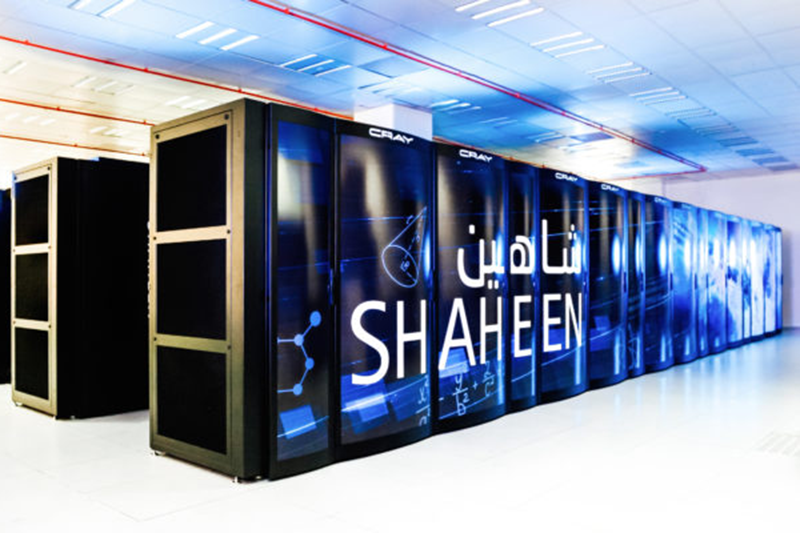
\includegraphics[width=0.6 \textwidth]{./Images/Shaheen-II.png}
    \end{center}
  \end{figure}
}

%*************************************************************************************

\section{Test Case Grid}

%*************************************************************************************

%-------------------------------------------------------------------------------------
\frame{
  \frametitle{Test Case Grid - Description}

  \begin{itemize}
  \item Fill grid (W = coef)
  \item L1 error between grid W and R 
  \item Get min. grid W
  \item Get max. grid W
  \item Update pressure W = 2*U - W + C*L (used in propagator)
  \item Medium Grid size 4 GB (1000 x 1000 x 1000 points)
  \end{itemize}
  
}

%-------------------------------------------------------------------------------------
\frame{
  \frametitle{Test Case Grid - Results}

  \begin{itemize}
  \item {\bf Machine: shaheen}
  \item 1 node / 32 threads
  \item CPU Baseline kernel and GPU kernels
  \end{itemize}
  
  {\scriptsize
  \begin{table}
    \caption{\scriptsize Bandwidth GB/s \footnote{\scriptsize \textcolor{blue}{Updated Dec 1, 2020}} }
    \label{table_memory}
    \begin{tabular}{@{}cccccc}
      Mode          & Fill & L1 err. & Get max. & Get min. & Update Pres. \\
      \hline
      Shaheen CPU   & 54   & 124     & 126      & 126      & 120 \\
      Ibex CPU      & 92   & 217     & 224      & 224      & 198 \\
      Ibex GPU1     & 92   & 217     & 224      & 224      & 198 \\
      Ibex GPU2     & 92   & 217     & 224      & 224      & 198 \\
      Ibex GPU3     & 92   & 217     & 224      & 224      & 198 \\
    \end{tabular}
  \end{table}
  }

  {\scriptsize
  \begin{table}
    \caption{\scriptsize Bandwidth GPoints/s}
    \label{table_memory}
    \begin{tabular}{@{}cccccc}
      Mode        & Fill & L1 err. & Get max. & Get min. & Update Pres. \\
      \hline
      Shaheen CPU & 13.5  & 15.5    & 31.5     & 31.5    & 6.0 \\
      Ibex CPU    & 23.0  & 27.1    & 56.0     & 56.0    & 9.9 \\
      Ibex GPU1   & 23.0  & 27.1    & 56.0     & 56.0    & 9.9 \\
      Ibex GPU2   & 23.0  & 27.1    & 56.0     & 56.0    & 9.9 \\
      Ibex GPU3   & 23.0  & 27.1    & 56.0     & 56.0    & 9.9 \\
    \end{tabular}
  \end{table}
  }

  Reproduce results with \texttt{./hackathonTestCases/testCase\_Grid/runMediumGridShaheen.sh}
  
  Elapsed few seconds.

}

%-------------------------------------------------------------------------------------
\frame{
  \frametitle{Test Case Grid - Summary}

  {\bf Machine: Shaheen}
  \begin{itemize}
  \item L1 Err., Get Min \& Max: 125 GB/s close to peak BW (92 \% Peak Mem. BW)
  \item {Low perf for Fill: 54-58 GB/s (40-43 \% Peak Mem. BW)}
  \item Max Err. 72-91 GB/s (53-67 \% Peak Mem. BW)
    \item Pressure update 6 GPoint/s (120 GB/s, 88 \% Peak Mem. BW)
  \end{itemize}
}

%*************************************************************************************

\section{Test Case Propa}

%*************************************************************************************

%-------------------------------------------------------------------------------------
\frame{
  \frametitle{Test Case Propa - Description}

  \begin{itemize}
  \item Seismic wave propagator
  \item 2nd order acoustic wave equation  
  \item Time-domain Finite-difference
  \item Various FD order in space
  \item 2nd FD order in time
  \item Various grid size and time steps
  \item Total 18 configurations
  \item Comparison against analytical solution (Eigen mode)
  \end{itemize}
  
}

%-------------------------------------------------------------------------------------
\frame{
  \frametitle{Test Case Propa - Results}
  
  \begin{itemize}
  \item {\bf Machine: shaheen}
  \item 1 node / 32 threads
  \item CPU Baseline kernel and GPU kernels \footnote{\scriptsize \textcolor{blue}{Updated Nov 28, 2020}}
  \item FD: Black O2, Blue O4, Pink O8, Red O12 / Square=CPU CacheBlk, Cross=GPU 
  \end{itemize}
  
  \begin{figure}
    \begin{center}
      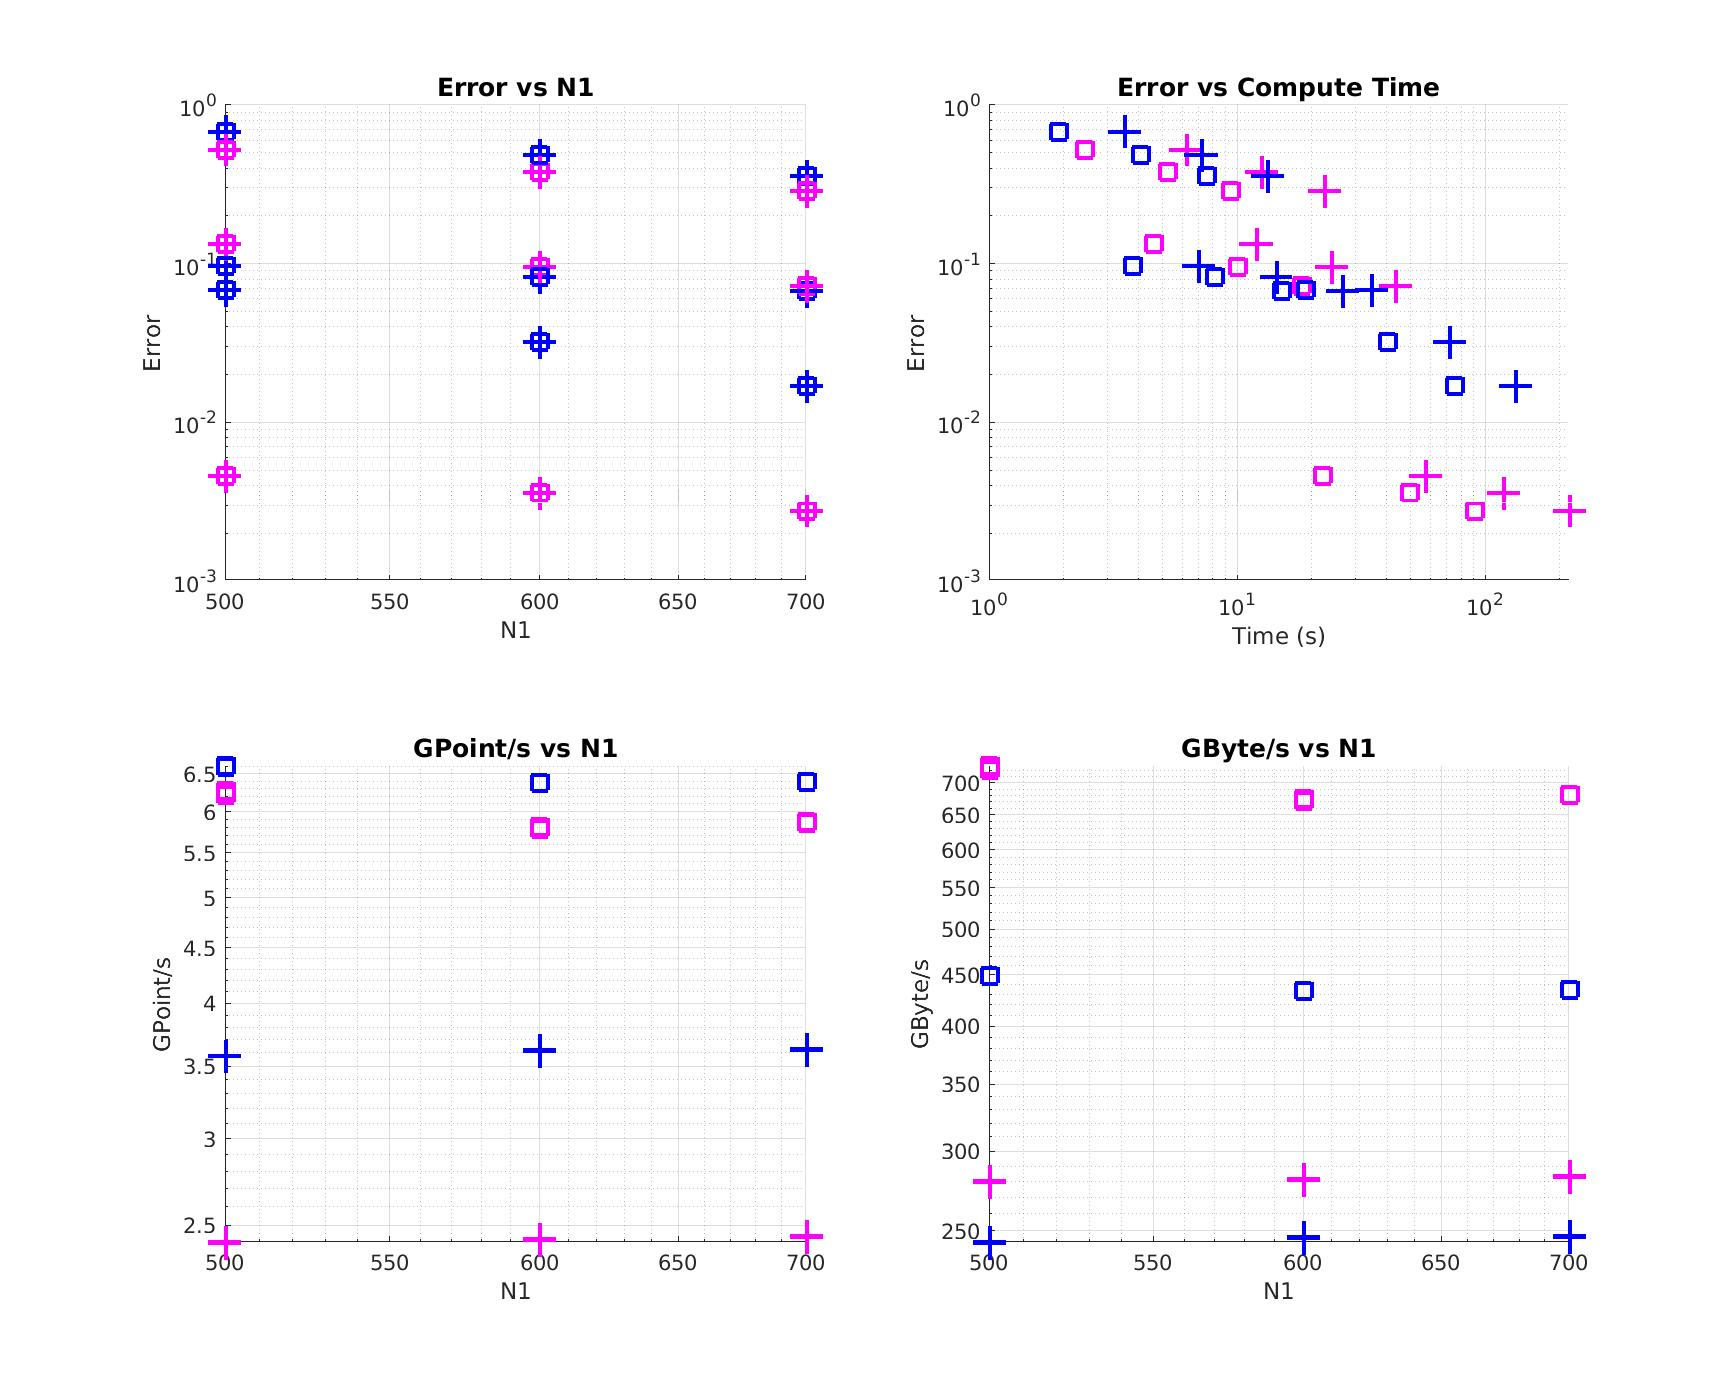
\includegraphics[width=0.6 \textwidth]{../../testCase_Propa/runShaheen.jpg}
    \end{center}
  \end{figure}

  Reproduce results with \texttt{./hackathonTestCases/testCase\_Propa/runShaheen.sh}
  
  Elapsed about an hour.

}

%*************************************************************************************

\section{Conclusions and next steps}

%*************************************************************************************

%-------------------------------------------------------------------------------------
\frame{
  \frametitle{Conclusions and next steps}

  TO DO
}

%*************************************************************************************

\section{Acknowledgements}

%*************************************************************************************

%-------------------------------------------------------------------------------------
\frame{
  \frametitle{Acknowledgements}

  \begin{itemize}
  \item KAUST ECRC and KSL for access and support on Shaheen II \& Ibex
  \end{itemize}
}

%-------------------------------------------------------------------------------------
%{\tiny{
%\def\newblock{\hskip .11em plus .33em minus .07em}
%\bibliographystyle{apalike}
%\bibliography{./biblioseiscope}
%}}

%\addtocounter{framenumber}{-4}

\end{document}

